% 原书印刷20--21页，PDF物理48--49页：从1.4标题开始.
\subsection{存在性的反例}\label{sec:1.4}\index{N112@最优映射的不存在性（non-existence of optimal maps）|hyperpage}

我们至少要给出两个不包含在\autoref{obj:1.17}的陈述之内、而且最优传输不存在的例子. 我们着重考虑这样的情形：成本$c(x,y)$通常允许我们得到存在性结果（例如取$c(x,y)=|x-y|^2$），但不存在性的原因在于测度$\mu$. 也可以构造不存在性由成本而非测度造成的其他例子；例如见\hyperref[ex:58]{习题58}和\hyperref[ex:59]{习题59}.

\subsubsection*{可能根本不存在传输}

第一个例子非常简单. 考虑$\mu=\delta_a$、$a\in X$的情形，并假设$\nu$不是Dirac质量. 此时根本没有传输映射. 事实上，容易验证$\mathrm{T}_\#\delta_a=\delta_{\mathrm{T}(a)}$；因此，如果$\nu$不能写成某个$b\in Y$对应的$\delta_b$，那么传输映射$\mathrm{T}:X\to Y$就不可能存在.

更一般地，对于$\mu$的每个原子$a$，像测度$\mathrm{T}_\#\mu$总包含一个质量至少为$\mu(\{a\})$的原子. 特别地，这意味着带原子的测度不能通过传输映射送到无原子的测度. 因此，当我们想求解(MP)时，源测度$\mu$无原子是一项典型假设.

相反，Kantorovich问题(KP)对于原子测度仍然有意义. 特别地，$\mu=\delta_a$时情形非常简单：集合$\Pi(\mu,\nu)$只有一个元素，即$\gamma=\mu\otimes\nu=\delta_a\otimes\nu$.

\subsubsection*{可以存在传输，但不存在最优传输}

考虑二次成本$c(x,y)=|x-y|^2$（但任何随距离严格递增的成本都会给出\mbox{相同结果）.} 令
\[
\mu=\mathscr H^1\mathbin{\vrule height 1.4ex depth -.3ex width .07ex\vrule height .07ex depth 0ex width .7ex}A,
\qquad
\nu=\frac{\mathscr H^1\mathbin{\vrule height 1.4ex depth -.3ex width .07ex\vrule height .07ex depth 0ex width .7ex}B+
\mathscr H^1\mathbin{\vrule height 1.4ex depth -.3ex width .07ex\vrule height .07ex depth 0ex width .7ex}C}{2},
\]
其中$A,B,C$是$\mathbb R^2$中三条相互平行的竖直线段，端点位于$y=0$与$y=1$两条直线上，横坐标分别为$0,1,-1$，而$\mathscr H^1$是一维Hausdorff测度（此例本质上来自\cite{b227}）. 显然，任何传输计划都不能实现比$1$更好的成本，因为每个点在水平方向上都必须移动距离$1$. 此外，把$A$分成$2n$条等长线段$(A_i)_{i=1,\ldots,2n}$，并把$B$和$C$各分成$n$条线段$(B_i)_{i=1,\ldots,n}$与$(C_i)_{i=1,\ldots,n}$（都按从上到下的顺序排列），便能得到映射序列$\mathrm{T}_n:A\to B\cup C$. 定义$\mathrm{T}_n$为分片仿射映射，把$A_{2i-1}$送到$B_i$，把$A_{2i}$送到$C_i$. 这样，映射$\mathrm{T}_n$的成本小于$1+1/n$，所以Kantorovich问题的下确界是$1$，只在传输映射中取下确界也得到$1$. 然而，没有映射$\mathrm{T}$能够取得成本$1$，因为这会要求所有点都沿水平方向移动，而这不能满足推前约束. 另一方面，与$\mathrm{T}_n$对应的传输计划弱收敛到
\[
\frac12\gamma_\mathrm{T}^++\frac12\gamma_\mathrm{T}^-,
\qquad \mathrm{T}^\pm(x)=x\pm e,\quad e=(1,0).
\]
这一传输计划实际上是唯一的最优传输计划，其成本为$1$.

注意，在最后这个例子中，我们还看到，传输映射中的下确界等于传输计划中的下确界（即最小值）. 这是一个依赖于松弛概念的一般事实，我们将在下一节看到.

\begin{center}
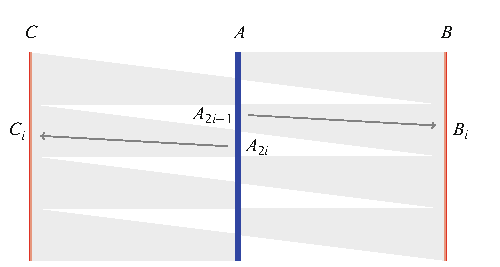
\includegraphics[width=.65\textwidth]{assets/fig-1-4-counterexample.pdf}
\end{center}
